% !TeX root = ./3-handout.tex

%possible excursion topics:
%bernadette's paradox, which i find puzzling, and relate briefly to causal explN; seems to me like Rayo and Yablo disagree about proper interpretation of this paradox! 
%causal explN background: e.g. woodward view (could be relevant for time-travel stuff, so could also save for later)
%rationality: straightforwardly factual vs. normative/plan-laden; defs relevant for decision theory unit!
%stuff on axiom of choice: relevant for bacon's puzzle
%could also save bacon puzzle for AoC unit! or return to later 
%could couple w/ Yablo's extension case, where the strategy to Bacon's paradox seems to lead to a genuine contradiction!!! see my notes in 3-thoughts and also the slides he sent me. Bevs vs. Owls 


% They could incorporate/do if needing to kill time:
% chalk and talk the review sheet for this week
% talk about the strangeness of reductio proofs (could do this in future as well!); but defs relevant this week given large number of reductio proofs on the pset 
%changes to notion of rigor in mathematics; e.g. bolzano moving away from physical intuition , motion, passage of time. 


%\newcounter{mysection}
%\setcounter{mysection}{1}
%\arabic{mysection}
%\roman{subsection}

%\begin{itemize}[<+->] 
%\item<2-> % reveals second and keeps on page in subsequent frames
%\begin{itemize}[<2->] %does for a whole list of items


\setcounter{section}{2} %sets section counter to 0. note that need to switch section counter from Roman to arabic for this to work! since no roman numeral for 0! %put this into preamble, i.e. file common.tex: \renewcommand\thesection{\arabic{section}}




\section{Omega Sequence Paradoxes}
%\subsection*{test}

\begin{frame}
%\large

\scriptsize{\tableofcontents}

\end{frame}


\begin{frame}
\frametitle{Liable to forget:}
%\large

\begin{itemize}[<+->]

\item PSet 3 has been posted! Due this Sunday 3/12, 5pm!

\item[] No quiz component this week: everything is a ``part 2'' justify your answers!

\item Feel free to join \href{https://piazza.com/mit/spring2023/24118}{Piazza}! 

\item Feel free to join PSet partners!!! 
\item[] Groups will be auto-assigned Friday


\end{itemize}
\end{frame}

\subsection{What are Paradoxes?}

\begin{frame}
\frametitle{What is a Paradox?}
%\large

\begin{itemize}[<+->]
% evidently
\item Evidently, we wait until 5 weeks in to tell you what this class is actually about!

\item \emph{Paradox}: an argument that appears to be valid and have true premises, yet leads to a seemingly false conclusion. Options:

\begin{enumerate}
\item show that the reasoning is invalid (denial) %Falsidical paradox
\item learn to live without one of the premises (rejection) %also a Falsidical paradox 
%i.e. one of the premises is false rather than true! 
\item learn to live with the conclusion (acceptance)
%i.e. the conclusion is actually true, not false! Instance of Quine's veridical paradox
\item Stuck: a true antinomy! 

\end{enumerate}
\bigskip
\item An \emphz{omega-sequence paradox} is a paradox based on an $\omega$-sequence ($| | | \dots$), so no last element \\ or a reverse $\omega$-sequence ($\dots | | | $), so no first element/beginning

\end{itemize}
\end{frame}

\begin{frame}
\frametitle{Zeno of Elea}
%\large

\begin{itemize}[<+->]

\item For all we know, Zeno of Elea's b-day could be today!

\item 5th century BCE Greece

\item Student of Parmenides: defender of monism 

\item Hence, in some sense, Zeno believed that he WAS Parmenides and that WE are all Zeno

\item So Zeno lives on, in the hearts and minds of the many, who are but one 

\end{itemize}
\end{frame}


\begin{frame}
\frametitle{Zeno's Paradox}
%\large

\begin{quote}
You wish to walk from point $A$ to point $B$. In order to do so, you must carry out an \(\omega\)-sequence of tasks:
\medskip
\begin{center}
\begin{tikzpicture}
\draw (0,0) -- (8,0); % line
\draw (4,0) -- (4,-0.2); %1/2 way mark
\node at (4,-0.5) {\scriptsize $\frac{1}{2}$};
\draw (6,0) -- (6,-0.2); %1/4 way mark
\node at (6,-0.5) {\scriptsize $\frac{3}{4}$};
\draw (7,0) -- (7,-0.2); %1/8 way mark
\node at (7,-0.5) {\scriptsize $\frac{7}{8}$};
\node at  (7.65,-0.5) {\dots};

\node at (-.3,0)  {$A$}; %  A
\draw[ultra thick] (0,0) circle [radius=.03];

\node at (8.3,0)  {$B$}; %  B
\draw[ultra thick] (8,0) circle [radius=.03];

\end{tikzpicture}
\end{center}
\[
\begin{array}{cc}
\pause \text{\scriptsize Task  1:} & \text{\scriptsize reach $\frac{1}{2}$ mark}\\
\pause \text{\scriptsize Task  2:} & \text{\scriptsize reach $\frac{3}{4}$ mark}\\
\pause \text{\scriptsize Task  3:} & \text{\scriptsize reach $\frac{7}{8}$ mark}\\
\pause \text{\tiny\vdots} & \text{\tiny\vdots}\\
\pause \text{\scriptsize Task  $n$:} & \text{\scriptsize reach $\frac{2^n-1}{2^n}$ mark}\\
\text{\tiny\vdots} & \text{\tiny\vdots}\\
\end{array}
\]

\pause 
But it's impossible to complete infinitely many tasks in a \\ finite amount of time. So \emph{movement is impossible}. 
\end{quote}
\end{frame}

\begin{frame}
\frametitle{Standard Response to Zeno}
%\large

\begin{itemize}[<+->]

\item Denial! the argument is invalid: 

\item At a speed of $1 m/s$, it takes $1$ second to walk a meter: the first task takes half a second, then a quarter of a second, then an eighth, then \dots $1/2^n$ seconds for the $nth$ task

\item $lim_{n \rightarrow \infty} (\frac{1}{2}+\frac{1}{4}+\frac{1}{8}+\dots + \frac{1}{2^n}) = lim_{n \rightarrow \infty} (1 - \frac{1}{2^n}) = 1$
%can do an inductive argument like in the book exercise, or use geometric series formula! 

\item \emph{Supertask}: complete countable-infinity of tasks in a finite time
%completing infinitely-many tasks in a finite time

\item Supertasks are physically possible provided that successive tasks take sufficiently less time
%i guess in this case, whenever a geometric series converges?
%take less and less time, converging to zero 

\item Alternatively, they would be physically possible if things could move arbitrarily fast, but here physics says ``nahhhh''

% % might want to note though that shadows can move infinitely fast! this might be in a supertask paper
%tachyons? 

\end{itemize}
\end{frame}



\subsection{Of Demons \& Rationality}

\begin{frame}
\frametitle{The Demon's Game}
%\large

In complete isolation, people \(P_1,P_2,P_3,\ldots\) take turns answering \\ \emph{aye} or \emphz{nay} (no one can coordinate on a strategy):

\begin{itemize}[<+->]

\item If exactly $n$ people say \emph{aye} ($n \in \mathbb{N}$), each person gets $\$n$. 

\item If infinitely many people say \emph{aye}, they all get nothing.

\item For an arbitrary speaker $P_k$, is there a unique \textit{rational} response?
%could do some meta-ethics on rationality, or save this for decision theory sessions!

\item It seems rational for $P_k$ to say \emph{aye}: she can't hurt anyone and might help everyone (if only finitely-many people say \emph{aye}, then $P_k$'s \emph{aye} contributes another dollar). 

\item \textbf{Puzzle}: But if it's rational for $P_k$, it's rational for everyone. \\ So nobody gets anything.

\end{itemize}
\end{frame}



\begin{frame}
\frametitle{Demon's Game Discussion}
%\large

\begin{itemize}[<+->]

\item Does rationality require each individual to say `aye'? 

\item Comparison: prisoner's dilemma

\item Does rationality require each prisoner to defect?

\item Can it be collectively rational for an individual(s) to behave irrationally? 

\end{itemize}
\end{frame}

\begin{frame}
\frametitle{Philosophy Prompt \#7}
%\large
Rationality says, ``plz attempt to answer all three questions":
\begin{enumerate}[<+->]

\item If you were placed within the Demon's Game, what would you answer and why?

\item If you had a friend in the Game, what would you want them to answer? Remember that you can't communicate with them before or during the game. 

\item Does \emph{rationality} require you to answer ``aye''? \\ i.e. are you \emphz{irrational} if you answer ``nay''? 

\medskip

\item[] {\small If exactly $n$ people say \emph{aye} ($n \in \mathbb{N}$), each person gets $\$n$.} 

\item[] {\small If infinitely many people say \emph{aye}, they all get nothing.}

\end{enumerate}
\end{frame}

\begin{frame}
\frametitle{Response 1: Acceptance}
%\large

\begin{itemize}[<+->]

\item Accept the conclusion: if every member behaves rationally, then no one makes any money

\item Motivation: for each individual, saying `aye'  \emph{weakly dominates}: it might increase how much money that individual makes, and it cannot decrease how much money they make 

\item[] (if infinitely-many others say `aye', $P_k$ saying `\emphz{nay}' won't change the result)

\item \textbf{Collective tragedy}: situations exist where in virtue of every member behaving rationally, the outcome is suboptimal for every group member

\item Implicit assumption: rationality requires following weak dominance reasoning 

\end{itemize}
\end{frame}

\begin{frame}
\frametitle{Response 2 (and 3): denial}
%\large

\begin{itemize}[<+->]

\item Instead, one could deny this implicit assumption. Reject that rationality requires following weak dominance reasoning

\item Perhaps rationality \textit{permits} but does not require choosing actions that weakly dominate

\item An alternative implicit premise one could deny: perhaps collective rationality does \textit{not} reduce to individual rationality

\item Argue that at the group-level, a rational response can require some individuals to behave \emphz{irrationally}
%note that this response will run into issues of action-guidance. will somehow need group members to coordinate so that they agree for some to be irrational
%seemingly this coordination is what can occur in the prisoner's dilemma (e.g. an iterated prisoner's dilemma)

\end{itemize}
\end{frame}

\subsection{Thomson's Lamp}

\begin{frame}
\frametitle{Thomson's Lamp}
%\large

You have a lamp with a toggle button: press the button once and the lamp goes on, press it again and the lamp goes off:
\[
\begin{array}{cc}
\text{\footnotesize Time to midnight} & \text{\footnotesize Status of lamp shortly thereafter} \\
\pause \text{\scriptsize 60$s$} & \text{\scriptsize off} \\
\pause \text{\scriptsize 30$s$} & \text{\scriptsize on}\\ %n = 0, so 2^{2*0+1} = 2^1
\pause \text{\scriptsize 15$s$} & \text{\scriptsize off}\\% n =1
\pause \text{\scriptsize 7.5$s$} & \text{\scriptsize on}\\ %n =1 

\text{\tiny\vdots} & \text{\tiny\vdots}\\
\pause \text{\scriptsize $\dfrac{60}{2^{2n}}s$} & \text{\scriptsize off}\\ %for evens
\text{\scriptsize $\dfrac{60}{2^{2n+1}}s$} & \text{\scriptsize on}\\%for odds; use same n here
\text{\tiny\vdots} & \text{\tiny\vdots}\\
\end{array}
\]
\pause 
Is the lamp on or off at midnight?

\end{frame}

\begin{frame}
\frametitle{Thomson's Lamp: Paradox}
%\large

\begin{itemize}[<+->]

\item For every time the lamp gets turned off before midnight, there is a later time before midnight when it gets turned on. 
\item[(C1):] \textbf{So the lamp can't be off at midnight}.

\item For every time the lamp gets turned on before midnight, there is a later time before midnight when it gets turned off. 
\item[(C2):] \textbf{So the lamp can't be on at midnight}.

\item[(P3):] But a lamp is either on or off. Otherwise, it's not a lamp!

\item[(C4):] So Thomson's `lamp' is not a lamp

\item Paradox: reject reasoning leading to C1 or C2 (denial); \\ reject P3 (rejection); or accept the conclusion C4

\end{itemize}
\end{frame}

\begin{frame}
\frametitle{Physical vs. Logical Impossibility}
%\large

\begin{itemize}[<+->]

\item \emphz{Physical Impossibility}: impossible according to the physical laws of  \textit{our world}

\item[] -- could still be metaphysically possible: possible according to the laws of some other possible world

\item \emph{Logically impossible}: impossible according to the axioms of a logical system

\item[] -- In most systems, contradictions are logically impossible 
\item[] -- It is logically impossible to raise your arm without moving it

\item Thomson's lamp is physically impossible (involves a button traveling faster than the speed of light), but it could be possible in worlds that allow objects to travel arbitrarily fast. 
%note that `arbitrarily fast' might be unbounded finite speeds. e.g. see exercise on p. 66: if button must travel fixed distance d, then you don't need button to travel infinitely fast. just arbitrarily large finite speeds. 

\item[] -- And it is definitely logically possible. 


\end{itemize}
\end{frame}

\begin{frame}
\frametitle{Response 1: Acceptance}
%\large

\begin{itemize}[<+->]

\item Accept that Thomson's lamp is not a lamp. 

\item This isn't to say that the object is logically impossible, just that we shouldn't think that such an object would really be a lamp

\item Structurally: we have an oscillating function that does not converge as time approaches midnight


\end{itemize}

 \begin{columns}
    \begin{column}{.4\textwidth}  
 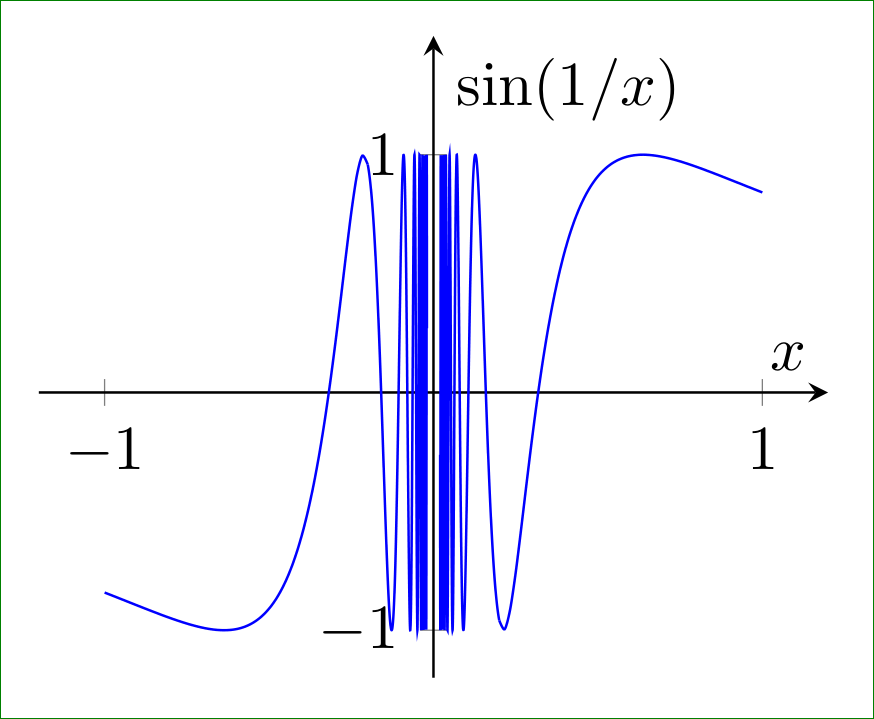
\includegraphics[height=.6\textheight]{../assets/sin_diverge}
    \end{column}
    \begin{column}{.6\textwidth}
\begin{itemize}[<+->]
\item Compare the function $sin(1/x)$: \\ the limits as $x$ goes to $0$ do not exist  \\ (oscillates between $1$ and $-1$)
%discontinuity at $x=0$

%note, function is undefined at x=0. so it is continuous on its domain. zero is outside the domain. but there is an essential discontinuity, since neither limit as x goes to zero from right or left exists 

\end{itemize}
  \end{column}
  \end{columns}

\end{frame}

\begin{frame}
\frametitle{Response 2: Denial}
%\large

\begin{itemize}[<+->]

\item Deny that the reasoning leading to C1, C2, or both is valid:

\item \small{``For every time the lamp gets turned off before midnight, there is a later time before midnight when it gets turned on.} 
\item[(C1):] \small{\textbf{So the lamp can't be off at midnight"}}

\item Notice that these arguments \textit{implicitly assume} that the lamp changes in a \emph{continuous} manner

\item But the lamp's on/off pattern could be \emphz{discontinuous}

\item Once we allow the `lamp' to change discontinously, the arguments are consistent with the lamp being on at midnight, and also consistent with the lamp being off at midnight
%Notice that these arguments are 

\item So it is logically possible that Thomson's lamp is actually on at midnight (x-or off at midnight). %Our argument doesn't settle the matter

\item How might a proponent of acceptance respond?

\end{itemize}
\end{frame}

\begin{frame}
\frametitle{A Rebuttal from Acceptance}
%\large

\begin{itemize}[<+->]

\item Defend a further premise P4:

\item[(P4):] Lamps work in a continuous manner: if the lamp is in a state $s$ at a given time $t$, then there must be states that are arbitrarily similar to $s$ at times sufficiently close to $t$

\item So Thomson's `lamp' is not a lamp

\item But notice that this response still grants the possibility that the object is definitively off (or definitively on) at midnight
% in some sense, this response still grants the main point of the denial proponent.
% Indeed, we might think what is really in question here is whether we should think that the object is neither off/on it midnight or if it is determinately off/on at midnight.

\item \emph{Moral}: sometimes paradoxes implicitly smuggle in physical assumptions that need to be made explicit to assess whether the situation is \textit{logically} paradoxical

\end{itemize}
\end{frame}




\subsection{Bomber Jackets}

\begin{frame}
  \frametitle{The Bomber's Paradox}

There are infinitely many bombs. Should one of the bombs go off, it will instantaneously disable all other bombs. \\ So a bomb goes off if and only if no bombs have gone off before it:

  \begin{columns}
    \begin{column}{.4\textwidth}  
 \[
\begin{array}{cc}
\text{\footnotesize Bomb} & \text{\footnotesize When bomb is set to go off} \\
\text{\scriptsize $B_0$} & \text{\scriptsize 12:00pm} \\
\text{\scriptsize $B_1$} & \text{\scriptsize 11:30am} \\
\text{\scriptsize $B_2$} & \text{\scriptsize 11:15am} \\
\text{\tiny\vdots} & \text{\tiny\vdots}\\
\text{\scriptsize $B_k$} & \text{\scriptsize \(\dfrac{1}{2^k}\) hours after 11:00am} \\
\text{\tiny\vdots} & \text{\tiny\vdots}\\
\end{array}
\]  
    \end{column}
    \begin{column}{.6\textwidth}
    \begin{itemize}
    {\scriptsize
\item Condition for a bomb to explode:\\[1.5ex]
\item[(0)] \(B_0\) goes off $\leftrightarrow$ \(B_n\)  fails to go off ($\forall n > 0$). \\[1.5ex]
\item[(1)] \(B_1\) goes off $\leftrightarrow$ \(B_n\)  fails to go off ($\forall n > 1$).  \\[1.5ex]
\item[(2)] \(B_2\) goes off $\leftrightarrow$ \(B_n\) fails to go off ($\forall n > 2$).

\hspace{5mm}\vdots

\item[(k)] \(B_k\) goes off $\leftrightarrow$ \(B_n\) fails to go off ($\forall n > k$).
\item[(k+1)] \(B_{k+1}\) goes off $\leftrightarrow$ \(B_n\) fails to go off ($\forall  n > k+1$).

\hspace{5mm}\vdots }
\end{itemize} 
    \end{column}
  \end{columns}
  Will any bombs go off?
\end{frame}

\begin{frame}
\frametitle{Bomber's Paradox: Arguments}
%\large
(\emph{k}): \(B_k\) goes off $\leftrightarrow$ \(B_n\) fails to go off ($\forall n > k$)

(\emphz{k+1}): \(B_{k+1}\) goes off $\leftrightarrow$ \(B_n\) fails to go off ($\forall  n > k+1$).
\begin{itemize}[<+->]

\item Consider an arbitrary bomb $B_k$; first we'll argue it can't go off; second we'll argue it must go off!

\item Suppose $B_k$ goes off. Then for each $n> k$, $B_n$ must fail to go off. Hence $B_{k+1}$ fails to go off and $\forall n > k+1$, $B_n$ fails to go off. 
\item[] But then $B_{k+1}$ must go off, in which case $B_k$ is disabled. 

\item Suppose $B_k$ fails to go off. Then by statement (k), $B_m$ must have gone off for some $m > k$. But then run the preceding argument to show this $B_m$ could not have gone off. Contradiction. 

\item So $B_k$ can neither go off nor fail to go off. 

\end{itemize}
\end{frame}

\begin{frame}
\frametitle{Response 1: Rejection}
%\large

\begin{itemize}[<+->]

\item Premise: the reverse omega sequence of bomb constraints (sentences (0), (1), \dots, (k), \dots) is logically consistent and hence jointly possible

\item Reject this premise: deny that the setup is logically possible

\item Essentially, argue that the set of these sentences is actually the empty set $\emptyset$

\end{itemize}
\end{frame}

\begin{frame}
\frametitle{An analogy to motivate Rejection}
%\large

\begin{itemize}[<+->]

\item Analogous situation: reverse omega sequence of barbers: \\ $\dots$, $B_{k+1}$, $B_k$, \dots, $B_2$, $B_1$,$B_0$
%$B_0$, $B_1$, $B_2$, \dots, $B_k$, \dots 

\item Analogous constraint $(\emph{k'})$: a barber cuts his own hair if and only if no prior barber has cut his own hair

\item Does barber $B_k$ cut his hair or not?
% Argument: if B_k cuts his hair, then no prior barber has cut his hair, so B_k+1 would have cut his hair, in which case B_k would not have cut his hair
% if B_k does not cut his hair, then some prior barber B_m cut his hair. but then run the preceding argument and get a contradiction. 

\item Rejection response: it is logically impossible for there to be a set of barbers that satisfy this condition

\item \emph{Broader moral}: ``unrestricted comprehension" fails: \\ just because you can write down a property doesn't mean it corresponds to a non-empty set (or even to a set at all) 
%we can write down properties that seem to refer to a non-empty set, actually do not refer to sets



\end{itemize}
\end{frame}

\begin{frame}
\frametitle{Response 2: Acceptance(?)}
%\large

\begin{itemize}[<+->]

\item If you are convinced that the setup is logically possible, then you are plausibly committed to the logical possibility of contradictions.

\item You seem to be committed to it being the case that $B_k$ goes off and it being the case that $B_k$ does not go off 

\item \emphz{Dialetheism}: some contradictions are true, \\ e.g. ``$p \eand \enot p$" is true for some proposition $p$

%from SEP on dialetheism: ``Dialetheism should, however, be clearly distinguished from paraconsistency. Whereas dialetheists must embrace some paraconsistent logic or other to avoid trivialism, paraconsistent logicians need not be dialetheists: they may subscribe to a non-explosive view of entailment for other reasons. Within paraconsistency, one may distinguish (at least) four grades of paraconsistent involvement"

%cool quote from Wittgenstein RFM:
%``Why should Russell’s contradiction not be conceived of as something supra-propositional, something that towers above the propositions and looks in both directions like a Janus head? The proposition that contradicts itself would stand like a monument (with a Janus head) over the propositions of logic (1978, III.59)."
\end{itemize}
\end{frame}

\begin{frame}
\frametitle{An Explanatory Puzzle about Response 1}
%\large

\begin{itemize}[<+->]

\item But a puzzle remains for the Rejection response: \\ what \textit{explains} why it is logically (and hence physically) impossible to construct this sequence of bombs?

\item Locally, any finite sequence of bombs can be programmed in the appropriate manner, and an infinite being could complete a supertask of programming infinitely-many bombs in finite time. 
%and any finite sequence could be arbitrarily extended to a longer finite sequence of such bombs. so in this sense we can program a potentially infinite sequence of such bombs. but not an actually infinite sequence

%moral on p. 72: our intutions are s.t. when a potential infinity is logically impossible, we feel that an actual infinity ought to be logically possible. 

\item What happens when an infinite being tries to program the bombs according to sentences (0), (1), \dots, (k), \dots? 

\item Something must stop them from succeeding, but what?

%we'll return to this with the grandfather paradox?

\end{itemize}
\end{frame}

\begin{frame}
\frametitle{Philosophy Prompt \#8: Benardete's Paradox}
%\large

\begin{itemize}[<+->]
\item You're trying to run from 0 to 1 meter. You're confronted by a reverse omega sequence of Gods, each placed at $\frac{1}{2^n}$.
\item Each God will raise a wall to block you if and only if you reach them (so iff no other God has blocked you yet)\\[1ex]


\includegraphics[height=.22\textheight]{../assets/Benardete}

\item Describe what happens or otherwise interpret this situation. \\ If you believe a certain event occurs (or not), what explains it? 

\end{itemize}
\end{frame}

\begin{frame}
\frametitle{Response 1: Blocked}
%\large

\begin{itemize}[<+->]

\item You're halted at $0$ meters. No particular God stops you (not a single wall is raised)

\item What explains why you can't get past $0$ meters?

\item Saying that `logic stops you' isn't very satisfying

\item Is there any \textit{causal} explanation to be had?

\item What is a \textit{causal explanation} anyways???

%34min: reverse omega sequence w/ walls and bullet; study this one! 
%student and rayo: case puts pressure on our ordinary thinking about causation. seemingly the bullet must be stopped immediately, but not by any particular wall.
%rayo: might show that our notions of causation are parochial. designed for kind of world we live in but not these other kinds of situations.
%reject idea that `if the bullet is stopped, then something stopped it''

%lecture 2, yablo around 11min. rewatch 

\end{itemize}
\end{frame}

\begin{frame}
\frametitle{Response 2: Smooth Sailing(?)}
%\large

\begin{itemize}[<+->]

\item Rejection: reject that the setup of the gods is logically possible

\item Just like in the Bomb-case, argue that although locally each God could carry-out its plan, collectively it is impossible for them to carry out the plan

\item So the Gods fail to enact their plan and you get past $0$ meters

\item But then couldn't one of the Gods still raise their wall? \\ In which case you might get stuck at any point? 

\end{itemize}
\end{frame}




\subsection{Yablo's Paradox}

\begin{frame}
 \frametitle{Yablo's Paradox}

  \begin{columns}
    \begin{column}{.6\textwidth}
    There are infinitely many sentences:
\[
\begin{array}{cc}
\text{\footnotesize Label} & \text{\footnotesize Sentence} \\
 \text{\scriptsize $S_0$} & \text{\scriptsize ``For each \(i>0\), sentence \(S_i\) is false''} \\
\text{\scriptsize $S_1$} & \text{\scriptsize ``For each \(i>1\), sentence \(S_i\) is false''} \\
\text{\scriptsize $S_2$} & \text{\scriptsize ``For each \(i>2\), sentence \(S_i\) is false''} \\
\text{\tiny\vdots} & \text{\tiny\vdots}\\
\text{\scriptsize $S_k$} & \text{\scriptsize ``For each \(i>k\), sentence \(S_i\) is false''} \\
\text{\tiny\vdots} & \text{\tiny\vdots}\\[2ex] 
\end{array}
\]
    \end{column}
    \begin{column}{.4\textwidth}
    \small{The sentence meanings guarantee that each of the following must be true:\\[1ex]}
    \begin{itemize}
    {\scriptsize
\item[(0)] \(S_0\) is true $\leftrightarrow$ \(S_n\) is false (\(n>0\)).\\[1.5ex]

\item[(1)] \(S_1\) is true $\leftrightarrow$ \(S_n\)  is false (\(n>1\)).\\[1.5ex]

\item[(2)] \(S_2\) is true $\leftrightarrow$ \(S_n\) is false (\(n>2\)).

\hspace{5mm }\vdots

\item[(k)] \(S_k\) is true $\leftrightarrow$ \(S_n\)  is false (\(n>k\)).
\item[(k+1)] \(S_{k+1}\) is true $\leftrightarrow$ \(S_n\)  is false (\(n>k+1\)).

\hspace{5mm }\vdots }
\end{itemize} 
    \end{column}
  \end{columns}
Which sentences are true and which ones are false?
\end{frame}

\begin{frame}
\frametitle{The Paradox in Yablo's Paradox}
%\large

\begin{itemize}[<+->]

\item[(k)] \(S_k\) is true $\leftrightarrow$ \(S_n\)  is false (\(n>k\)).
\item[(k+1)] \(S_{k+1}\) is true $\leftrightarrow$ \(S_n\)  is false (\(n>k+1\)).

\item Consider an arbitrary sentence \(S_k\). Suppose it is true:

\item Then by condition (k), $S_n$ is false for all $n> k$. \\ So then $S_{k+1}$ and all $S_n$ for $n > k+1$ are false. 
\item[] But then statement $S_{k+1}$ must actually be true by condition (k+1). Contradiction

\item By the preceding argument, $S_m$ is false for each arbitrary $m$. Picking a $k$, this shows that $S_m$ is false for each $m>k$. 
\item[] But then by (k), $S_k$ is true. Contradiction. 
%So suppose that for arbitrary $k$, sentence $S_k$ is false. Since $k$ is arbitrary,  $S_m$ is false for every $m> k$

\end{itemize}
\end{frame}

\begin{frame}
\frametitle{Yablo vs. the Bomber}
%\large

\begin{itemize}[<+->]

\item Two intertranslatable paradoxes; can we give same response(s)?

\item Perhaps less clear why/whether the set of Yablo sentences \\ ``(0), (1), \dots, (k), \dots" is logically impossible

%\item Easier to see that a set of bombs might be logically impossible to program bombs in a certain way. 

\item Whereas we concluded we couldn't program the bombs (something would stop us), what do we conclude here?

\item An infinite being could clearly write down all the Yablo sentences, \textit{qua} marks on a page

\item So in what sense do these sentences `fail to exist'? 

%We can clearly write them all down, but they are not jointly satisfiable

\item \textit{Possible answer}: In a consistent bivalent logic, there is no model that assigns them all truth-values. \\ In that sense, the set is logically impossible: not meaningful
% So perhaps misleading to just say that there is no model that makes them all true 

\item Models exist that assign truth-values to an arbitrarily large finite number of Yablo sentences, but not all of them. 

% % So perhaps I don't find Yablo's puzzle really any more puzzling than the bomber paradox.

% % See bottom of page 76 four Rayo interpretation/response to Yablo's paradox. He modifies his semantic localist response to the liar paradox. Perhaps this is subtly different in some ways from what I have said above. He is arguing that the Yablo sentences must remain uninterpreted: neither true nor false). tried to fix my response above to accommodate this. 


\end{itemize}
\end{frame}

\subsection{The Three Prisoners Puzzle}

\begin{frame}
\frametitle{The Three Prisoners}
%\large

\begin{itemize}[<+->]

\item Three prisoners: Each of them is assigned a red or blue hat, based on the outcome of a coin toss.
\item Each of them can see the colors of the others' hats but has no idea about the color of his own hat.
\item The prisoners are taken into separate cells and asked about the color of their hat. They can offer an answer or remain silent. 
\medskip
\begin{itemize}
\item If all three prisoners remain silent, all three will remain captive %be killed.
\item If one of them answers incorrectly, all three will remain captive %be killed.
\item If at least one prisoner offers an answer, and everyone who offers an answer answers correctly, then all three prisoners will be freed.
\end{itemize}
\medskip
\item \emph{Puzzle}: Find a strategy that the prisoners could agree upon ahead of time that would guarantee that their chance of survival is above 50\%.

\end{itemize}
\end{frame}

\begin{frame}
\frametitle{A Strategy for the Three Prisoners}
%\large

\begin{itemize}[<+->]

\item Have each prisoner follow these instructions:

\item[a)] If the other two prisoners have hats of the same color, answer the guard by saying the opposite color

\item[b)] If the other two prisoners have different color hats, remain silent

\item Result: 75\% chance of being freed! 

\item Remains the case that each prisoner individually has only a 50\% chance of answering correctly (out of eight possibilities, they remain silent in four, answer correctly in two, \& incorrectly in two)

\item \emph{Moral}: by coordinating on a strategy, a group can improve the chance of collective success without changing chance of individual success

\end{itemize}
\end{frame}

\begin{frame}
\frametitle{Illustrating the Strategy}
%\large

\begin{itemize}[<+->]
\item The eight possible hat distributions, along with the result of applying the suggested strategy: 
\end{itemize}

\[
\begin{array}{cccc}
\text{\footnotesize Prisoner $A$} & \text{\footnotesize Prisoner $B$} & \text{\footnotesize Prisoner $C$} &\text{\footnotesize Result of following Strategy} \\
 \text{\scriptsize red} & \text{\scriptsize red} & \text{\scriptsize red} & \text{\scriptsize Everyone answers incorrectly} \\
  \text{\scriptsize red} & \text{\scriptsize red} & \text{\scriptsize blue} & \text{\scriptsize $C$ answers correctly} \\
   \text{\scriptsize red} & \text{\scriptsize blue} & \text{\scriptsize red} & \text{\scriptsize $B$ answers correctly} \\
    \text{\scriptsize red} & \text{\scriptsize blue} & \text{\scriptsize blue} & \text{\scriptsize $A$ answers correctly} \\
     \text{\scriptsize blue} & \text{\scriptsize red} & \text{\scriptsize red} & \text{\scriptsize $A$ answers correctly} \\
      \text{\scriptsize blue} & \text{\scriptsize red} & \text{\scriptsize blue} & \text{\scriptsize $B$ answers correctly} \\
       \text{\scriptsize blue} & \text{\scriptsize blue} & \text{\scriptsize red} & \text{\scriptsize $C$ answers correctly} \\
        \text{\scriptsize blue} & \text{\scriptsize blue} & \text{\scriptsize blue} & \text{\scriptsize Everyone answers incorrectly} \\
\end{array}
\]
\end{frame}

\subsection{Bacon's Puzzle}

\begin{frame}
\frametitle{Bacon's Puzzle}
%\large

\begin{itemize}[<+->]

\item An omega sequence of prisoners: \(P_1,P_2,P_3,\dots\). (\(P_1\) is at the end of the line, in front of her is \(P_2\), in front of him is \(P_3\), and so forth.) 

\item Each person is assigned a red or blue hat, based on the outcome of tossing a fair coin. 

\item Everyone can see the hats of the people in front of her, but cannot see her own hat (or the hat of anyone behind her). 

\item At a set time, everyone has to guess the color of their own hat by crying out ``Red!" or ``Blue!".

\item People who correctly call out the color of their own hats will be freed. Everyone else will remain captive. 

\item \emph{Puzzle}: Find a strategy that \(P_1, P_2, P_3, \ldots\) could agree upon in advance that would guarantee that at most finitely many people remain captive. 

\end{itemize}
\end{frame}

\begin{frame}
\frametitle{A Solution to get that bacon}
%\large

\begin{itemize}[<+->]
\item Use the Axiom of Choice (duh!)

\item Partition the set of all $\omega$-sequences of $0$s and $1$s

\item Two sequences belong to the same equivalence class provided they disagree at only finitely-many positions

\item For each equivalence class, the prisoners agree on a representative from that equivalence class (using AoC)

\item Each prisoner can determine which equivalence class the line belongs to (since they see infinitely-many hats in front of them and only finitely-many hats are behind)

\item \textit{Strategy}: answer assuming that the actual sequence is described by the chosen representative

\item The prisoners are guaranteed to be wrong only about finitely-many positions


\end{itemize}
\end{frame}

\begin{frame}
\frametitle{Magic Bacon?}
%\large

\begin{itemize}[<+->]
\item What is happening? Individually, each prisoner has at best a 50\% chance of guessing their hat-color correctly

\item Somehow, following this strategy \textit{guarantees} that only finitely-many prisoners remain captive

\item What is the probability that any individual who follows this strategy correctly calls out their hat color?
% See page 84. Rayo argues that this probability is not defined. Might need to look into stuff on non-measurable sets coming from axiom of choice


\end{itemize}
\end{frame}



\begin{frame}
  \frametitle{Liable to forget!}

      \begin{itemize}[<+->]
        \item remember to discuss word limit on PSet 3!

%\item Might want to model the kind of explN we're looking for in the prisoner's problem: coordination explains things. so this is a reason to leave bacon's puzzle till the very end and do three hats first. since three hats is harder version of  the HW problem 
      
      \end{itemize}
   
\end{frame}



















